\section{Quartic: degree=4}
\label{sec.quartic}

\subsection{Objectives}
The assignment in this section is:
\begin{enumerate}
\item Complete the file \code{src/quartic.py} by writing a Python
  function which computes and returns the x-intercepts of a curve
  equation is \[y=a x^4 + b x^3 + c x^2 + d x + e\,.\]
\item You'll need to replace all occurances of \code{raise NotImplementedError()}
  with correct python code which passes the tests.
\item Test the function in GitHub Codespaces by running the file\\
  \code{test/test\_quartic.py}.
\end{enumerate}

\subsection{Overview}


A polynomial of degree 4 has the form $P(x) = a x^4 + b x^3 + c x^2 + d x + e$. If $a=0$ than $P(x)$ is really
a cubic polynomial (degree 3) and can be solved using the techniques described in Section~\ref{sec.cubic}.

Two quartic equations (for $P_1(x)$ and $P_2(x)$) are plotted in Figure~\ref{fig.quartic}.

\begin{figure}
\centering
%% derived from https://tex.stackexchange.com/questions/357538/graph-of-a-parabola-on-pgfplots
%% Thanks to Stefan Pinnow
%%     https://tex.stackexchange.com/users/95441/stefan-pinnow

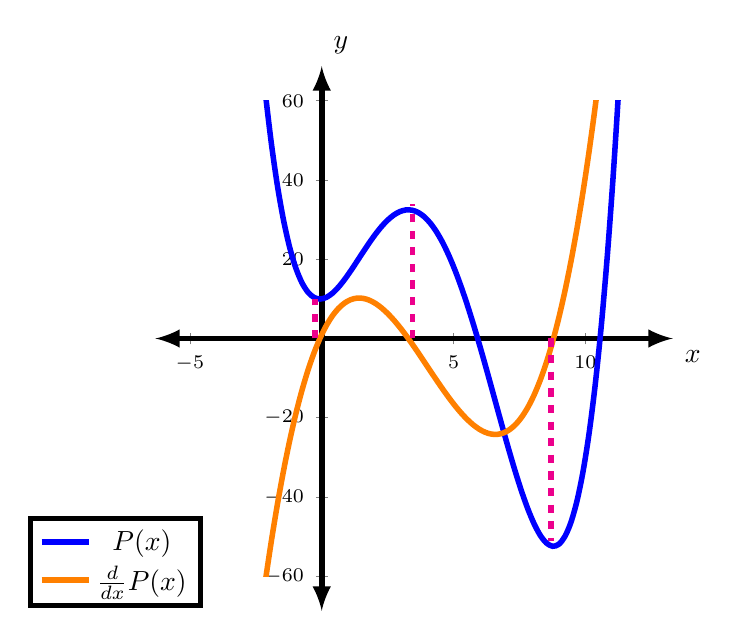
\begin{tikzpicture}
  \begin{axis}[
      samples=70,
      smooth,
      line width=2pt,
      domain=-4:12,
      legend pos=south west,
      legend style={
        anchor=east
      },
      width=0.6\textwidth,
      height=3in,
      axis lines=middle,
      xmin=-5,
      xmax=12,
      ymin=-60,
      ymax=60,
        scaled ticks=false,
        ticklabel style={font=\scriptsize},
        xlabel=$x$,
        ylabel=$y$,
        axis line style={
          latex-latex,
          shorten >=-12.5pt,
          shorten <=-12.5pt,
        },
        xlabel style={at={(ticklabel* cs:1)}, xshift=12.5pt, anchor=north west},
        ylabel style={at={(ticklabel* cs:1)}, yshift=12.5pt, anchor=south west},
    ]
    
    \addplot[color=blue] {0.125 * x^4 -2* x^3 + 7 * x^2 + x + 10};  
    \addlegendentry{\(P(x)\)}
    \addplot[color=orange] {0.5 * x^3 -6* x^2 + 14 * x + 1};
    \addlegendentry{\(\frac{d}{dx}P(x)\)}
    \draw[dashed,line width=1pt,line width=2pt,color=magenta] (3.45,0) -- (3.45,34);
    \draw[dashed,line width=1pt,line width=2pt,color=magenta] (8.7,0) -- (8.7,-51);
    \draw[dashed,line width=1pt,line width=2pt,color=magenta] (-0.25,0) -- (-0.25,10);
  \end{axis}
\end{tikzpicture}
%

\caption{Quartics}
\label{fig.quartic}
\end{figure}

\begin{align*}
  P_1(x) &= \frac{1}{8}  x^4 -2 x^3 + 7  x^2 + x + 6\\
  P_2(x) = -P_1(x) &= -\frac{1}{8}  x^4 +2 x^3 - 7  x^2 - x - 6\\
  \frac{d}{dx} P_1(x) &= \frac{1}{2} * x^3 -6* x^2 + 14 * x + 1
\end{align*}
